\mainchapter{Revisión sistemática de la literatura}{\topbanner}\label{cap:revision-literatura}
\vspace*{0.7cm}

En esta sección se describe el proceso de revisión sistemática de la literatura aplicado para identificar, seleccionar y analizar la evidencia científica relevante al dominio de estudio. Siguiendo la metodología propuesta por \citet{Sepulveda2021}, se definieron las bases teóricas del mapeo y se establecieron preguntas de investigación que guiaron la búsqueda en cinco bases de datos científicas, complementada con la técnica de \textit{snowballing}. A partir de este proceso se conformó un conjunto final de 22 estudios que sustentan las decisiones adoptadas en las etapas posteriores de la investigación.

\section{Construcción de la bitácora}\label{sec:construccion-bitacora}

Con el propósito de establecer una base teórica sólida que permitiera sustentar la toma de decisiones respecto a la selección de un servicio de directorio, se llevó a cabo una revisión exhaustiva de la literatura relacionada con el tema. Este proceso se desarrolló en diferentes etapas, las cuales se describen a continuación:


\subsection{Planeación}\label{subsec:planeacion}

El objetivo de esta etapa fue definir el propósito general del \ac{SMS}, adoptando la metodología propuesta por \citet{Sepulveda2021}. A su vez, se definieron metas (ver \autoref{tab:metas}), preguntas de investigación (ver \autoref{tab:preguntas}) y métricas (ver \autoref{tab:metricas}). Para ello, se siguió el modelo Objetivo-Pregunta-Métrica (\acs{GQM}).


\subsubsection{Definición de metas para el \texorpdfstring{\ac{SMS}}{SMS}}
\begin{table}[H]
	\centering
	\caption{Definición de metas del \acs{SMS}}
	\label{tab:metas}

	\renewcommand{\arraystretch}{1.2}
	\fontsize{9pt}{10pt}\selectfont

	\begin{tabularx}{\textwidth}{|c|X|}
		\hline
		\textbf{Meta} &
		\textbf{Descripción}
		\\
		\hline
		G1            &
		Identificar trabajos acerca de herramientas tecnológicas relacionadas con servicios de directorio de código abierto/software libre.
		\\
		\hline
		G2            &
		Analizar y clasificar las herramientas tecnológicas relacionadas con servicios de directorio de código abierto según sus características técnicas, arquitectónicas y casos de uso reportados.
		\\
		\hline
	\end{tabularx}
\end{table}



\subsubsection{Definición de preguntas de investigación}\label{subsubsec:rq-def}
\begin{table}[H]
	\centering
	\caption{Definición de preguntas de investigación del \acs{SMS}}
	\label{tab:preguntas}

	\renewcommand{\arraystretch}{1.2}
	\fontsize{9pt}{10pt}\selectfont

	\begin{tabularx}{\textwidth}{|c|c|X|X|}
		\hline
		\textbf{Meta}                                                                                                                                                                                 &
		\textbf{Pregunta}                                                                                                                                                                             &
		\textbf{Descripción}                                                                                                                                                                          &
		\textbf{Motivación}
		\\
		\hline
		G1                                                                                                                                                                                            &
		Q1                                                                                                                                                                                            &
		\textit{¿Qué herramientas tecnológicas de código abierto se relacionan con servicios de directorio?}                                                                                          &
		\textbullet\ Identificar las soluciones de servicios de directorio de código abierto existentes en la literatura

		\textbullet\ Reconocer cuáles tecnologías han sido más estudiadas o utilizadas en distintos contextos.
		\\
		\hline
		G2                                                                                                                                                                                            &
		Q2                                                                                                                                                                                            &
		\textit{¿Cuáles son las características técnicas, arquitectónicas y los contextos de aplicación de las herramientas tecnológicas relacionadas con servicios de directorio de código abierto?} &
		\textbullet\ Reconocer cómo están estructuradas arquitectónica y técnicamente las soluciones de servicios de directorio de código abierto.

		\textbullet\ Identificar las características funcionales y técnicas más relevantes reportadas.

		\textbullet\ Analizar los contextos de aplicación y tendencias de uso de estas soluciones.
		\\
		\hline
	\end{tabularx}
\end{table}



\subsubsection{Definición de métricas}
\begin{table}[H]
	\centering
	\caption{Definición de métricas del \acs{SMS}}
	\label{tab:metricas}

	\renewcommand{\arraystretch}{1.2}
	\fontsize{9pt}{10pt}\selectfont

	\begin{tabularx}{\textwidth}{|c|X|}
		\hline
		\textbf{Métrica} &
		\textbf{Descripción}
		\\
		\hline
		M1               &
		Frecuencia de aparición de cada herramienta tecnológica.
		\\
		\hline
		M2               &
		Frecuencia de características técnicas y arquitectónicas reportadas en las herramientas tecnológicas.
		\\
		\hline
	\end{tabularx}
\end{table}


\newpage
\section{Búsqueda de estudios}

Esta etapa comprendió las siguientes secciones:
\begin{enumerate}
	\item Estrategia de búsqueda, ya sea independiente o combinada;
	\item Identificación general de estudios;
	\item Revisión de estudio; y finalmente,
	\item Selección de estudios para incluir en el \ac{SMS}.
\end{enumerate}


\subsection{Estrategia de búsqueda}\label{subsec:estrategia-busqueda}

La estrategia de búsqueda empleada en este estudio combinó consultas estructuradas en bases de datos científicas con la técnica de búsqueda en bola de nieve (\textit{snowballing}). Esta integración metodológica permitió ampliar el alcance del proceso de identificación de literatura relevante, favoreciendo la recuperación de estudios adicionales a partir de las referencias bibliográficas y citaciones de los trabajos inicialmente seleccionados. Como resultado, fue posible identificar investigaciones de interés que podrían no haber sido localizadas mediante la aplicación exclusiva de estrategias de búsqueda tradicionales, fortaleciendo así la exhaustividad y cobertura del mapeo sistemático.


\subsection{Búsqueda en bases de datos}\label{subsec:busqueda-bases-datos}

Para la realización del \ac{SMS}, se seleccionaron las bases de datos Web of Science, IEEE Xplore, Springer, ScienceDirect y Taylor \& Francis. La elección de estas fuentes se fundamentó en su reconocida relevancia dentro de la comunidad científica, así como en la amplitud y calidad de la literatura que indexa en el área de investigación objeto de estudio. Adicionalmente, su disponibilidad y cobertura temática permitieron garantizar el acceso a publicaciones científicas actualizadas y pertinentes, contribuyendo a la rigurosidad y confiabilidad del proceso de búsqueda y selección de la evidencia científica.


\subsubsection{Identificación de estudios mediante búsqueda en bases de datos}\label{subsubsec:identificacion-estudios}

En esta etapa fue necesario definir un marco de referencia que facilitara la identificación y selección de las palabras clave más adecuadas para la construcción de la cadena de búsqueda empleada en las bases de datos seleccionadas. Con este propósito, se utilizó el modelo \ac{PICOC} como guía metodológica para estructurar y delimitar los términos de búsqueda relacionados con el objeto de estudio. La aplicación de este modelo permitió sistematizar el proceso de definición de palabras clave, favoreciendo la consistencia y trazabilidad de la estrategia de búsqueda. El resultado de este procedimiento se presenta en las \autoref{tab:modelo-picoc} y \autoref{tab:palabras-clave-picoc}.

\begin{table}[H]
	\centering
	\caption{Modelo \acs{PICOC}}
	\label{tab:modelo-picoc}

	\renewcommand{\arraystretch}{1.2}
	\fontsize{9pt}{10pt}\selectfont

	\begin{tabularx}{\textwidth}{|c|X|}
		\hline
		\tableheader
		\textbf{Componente} &
		\textbf{Descripción}
		\\
		\hline
		Población           &
		Estudios relacionados con los servicios de directorio
		\\
		\hline
		Intervención        &
		Observación y tabulación.
		\\
		\hline
		Comparación         &
		Identificación de características técnicas y arquitectónicas reportadas en las herramientas tecnológicas.
		\\
		\hline
		Salidas             &
		Conjunto de herramientas tecnológicas de servicios de directorio de código abierto y sus características técnicas y arquitectónicas.
		\\
		\hline
		Contexto            &
		Gestión institucional, servicios de directorio, seguridad, autenticación e identidad.
		\\
		\hline
	\end{tabularx}
\end{table}

\begin{table}[H]
	\centering
	\caption{Palabras clave identificadas usando el modelo PICOC}
	\label{tab:palabras-clave-picoc}

	\renewcommand{\arraystretch}{1.2}
	\fontsize{9pt}{10pt}\selectfont

	\begin{tabularx}{\textwidth}{|c|X|}
		\hline
		\textbf{Categoría PICOC}         &
		\textbf{Palabras clave}
		\\
		\hline
		\textbf{Población}               &
		Directory services, Identity management systems, Authentication systems, Authorization systems, LDAP systems
		\\
		\hline
		\textbf{Intervención}            &
		Open source directory service, Free software, OpenLDAP, Open source identity management, LDAP implementation
		\\
		\hline
		\textbf{Criterios de aceptación} &
		Proprietary directory service, Commercial solutions, Active Directory
		\\
		\hline
		\textbf{Salidas}                 &
		Technical characteristics, Software architecture, Scalability, Security, Interoperability
		\\
		\hline
		\textbf{Contexto}                &
		Distributed infrastructure, Research infrastructure, Academic environment
		\\
		\hline
	\end{tabularx}
\end{table}


Los términos de búsqueda identificados a partir del modelo \ac{PICOC} y presentados en la \autoref{tab:palabras-clave-picoc} fueron complementados mediante la incorporación de sinónimos y conceptos relacionados, con el fin de ampliar la cobertura y sensibilidad del proceso de recuperación de estudios. El conjunto resultante de términos se muestra en la \autoref{tab:palabras-clave}. Estos términos constituyeron la base para la cadena de búsqueda utilizada en cada una de las bases de datos seleccionadas.

\begin{table}[H]
	\centering
	\caption{Palabras clave para la búsqueda en bases de datos}
	\label{tab:palabras-clave}

	\renewcommand{\arraystretch}{1.2}
	\fontsize{9pt}{10pt}\selectfont

	\begin{tabularx}{\textwidth}{|c|X|}
		\hline
		\tableheader
		\textbf{Palabra clave}     &
		\textbf{Sinónimos}
		\\
		\hline
		\textbf{Directory service} &
		Directory services, Network directory service, User directory
		\\
		\hline
		\textbf{LDAP}              &
		Lightweight Directory Access Protocol, LDAP-based system, LDAP directory service
		\\
		\hline
	\end{tabularx}
\end{table}


Con el objetivo de filtrar los resultados obtenidos y centrar el análisis en estudios relevantes para la investigación, se definieron criterios de inclusión y exclusión, los cuales se presentan en la \autoref{tab:criterios-inclusion-exclusion}. Estos criterios orientaron el proceso de selección de estudios, permitiendo identificar aquellos trabajos alineados con objetivos del \ac{SMS} y descartar aquellos que no contribuían de manera significativa a la respuesta de las preguntas de investigación ni al desarrollo del análisis.

\begin{table}[H]
	\centering
	\caption{Criterios de inclusión y exclusión}
	\label{tab:criterios-inclusion-exclusion}

	\renewcommand{\arraystretch}{1.2}
	\fontsize{9pt}{10pt}\selectfont

	\begin{tabularx}{\textwidth}{|c|X|X|}
		\hline
		\textbf{Categoría}                                                         &
		\textbf{Inclusión}                                                         &
		\textbf{Exclusión}
		\\
		\hline
		Campos                                                                     &
		Resumen, título y palabras clave.                                          &
		Documento completo
		\\
		\hline
		Tipo de publicación                                                        &
		Artículos, libros, capítulos de libros y actas de congresos.               &
		Tesis
		\\
		\hline
		Área/Disciplina                                                            &
		Administración, ciencias de la computación y tecnología de la información. &
		Áreas no relacionadas con la administración, las ciencias de la computación, las tecnologías de la información y la gestión.
		\\
		\hline
		Periodo                                                                    &
		Entre 2020 y 2026                                                          &
		Menos de 2020
		\\
		\hline
		Idioma                                                                     &
		Inglés y Español                                                           &
		---
		\\
		\hline
	\end{tabularx}
\end{table}



\subsubsection{Búsqueda en bases de datos}\label{par:busqueda-bases-datos}

La cadena de búsqueda correspondiente a cada una de las bases de datos seleccionadas se presenta en la \autoref{tab:cadena-busqueda}.

\begin{table}[H]
	\centering
	\caption{Cadena de búsqueda}
	\label{tab:cadena-busqueda}

	\renewcommand{\arraystretch}{1.2}
	\fontsize{9pt}{10pt}\selectfont

	\begin{tabularx}{\textwidth}{|X|}
		\hline
		\tableheader
		\textbf{Cadena de búsqueda} \\
		\hline
		(``Directory service'' OR ``Directory services'' OR ``User directory'') AND (``LDAP'' OR ``Lightweight Directory Access Protocol'' OR ``LDAP-based system'')
		\\
		\hline
	\end{tabularx}
\end{table}




\subsubsection{Métricas de la búsqueda sin criterios de inclusión/exclusión}\label{subsubsec:resumen-busqueda}

La \autoref{tab:bases-sin-exclusion} presenta la cantidad de publicaciones recuperadas en las bases de datos consultadas durante la búsqueda inicial, previa a la aplicación de los criterios de inclusión y exclusión. En esta etapa se identificaron un total de 1720 registros, distribuidos entre IEEE Xplore (39), \ac{WOS} (10), Springer (1019), Taylor \& Francis (38) y ScienceDirect (614). El detalle de esta búsqueda preliminar se presenta en el apéndice \ref{sec:busqueda-sin-criterios}.

\begin{table}[H]
	\centering
	\caption{Resultados de la búsqueda sin exclusión}
	\label{tab:bases-sin-exclusion}

	\renewcommand{\arraystretch}{1.2}
	\fontsize{9pt}{10pt}\selectfont

	\begin{tabularx}{\textwidth}{|X|c|c|c|>{\centering\arraybackslash}m{1.5cm}|c|c|}
		\hline
		\tableheader
		\textbf{Criterios}                               &
		\textbf{IEEE}                                    &
		\textbf{WOS}                                     &
		\textbf{Springer}                                &
		\textbf{Taylor \& Francis}                       &
		\textbf{ScienceDirect}                           &

		\textbf{Total}
		\\
		\hline
		Cadena de búsqueda con palabras clave únicamente &
		39                                               &
		10                                               &
		1019                                             &
		38                                               &
		614                                              &
		1720
		\\
		\hline
		Contribución porcentual                          &
		2,27\%                                           &
		0,58 \%                                          &
		59,24\%                                          &
		2,21\%                                           &
		35,70\%                                          &
		100\%
		\\
		\hline
	\end{tabularx}
\end{table}



\subsubsection{Métricas de la búsqueda con criterios de inclusión/exclusión}\label{subsec:resumen-busqueda-citerios}

Esta búsqueda aplicó los criterios de inclusión y exclusión previamente definidos. Si bien se utilizó la misma cadena de búsqueda, esta etapa se diferencia por la aplicación de filtros específicos en cada base de datos. Las evidencias correspondientes a este proceso pueden consultarse en el apéndice~\ref{sec:busqueda-con-criterios}.

La \autoref{tab:bases-con-exclusion} presenta los resultados obtenidos tras la aplicación de los criterios de inclusión y exclusión. En contraste con la búsqueda inicial, en esta fase los filtros aplicados redujeron de manera significativa la cantidad de publicaciones recuperadas. En total, se identificaron 159 documentos, distribuidos de la siguiente manera: IEEE Xplore (3), \ac{WOS} (1), Springer (132), Taylor \& Francis (1) y ScienceDirect (22).

\begin{table}[H]
	\centering
	\caption{Resultados de la búsqueda con criterios de exclusión}
	\label{tab:bases-con-exclusion}

	\renewcommand{\arraystretch}{1.2}
	\fontsize{9pt}{10pt}\selectfont

	\begin{tabularx}{\textwidth}{|X|c|c|c|>{\centering\arraybackslash}m{1.5cm}|c|c|}
		\hline
		\tableheader
		\textbf{Criterios}                                        &
		\textbf{IEEE}                                             &
		\textbf{WOS}                                              &
		\textbf{Springer}                                         &
		\textbf{Taylor \& Francis}                                &
		\textbf{ScienceDirect}                                    &

		\textbf{Total}
		\\
		\hline
		Cadena de búsqueda con criterios de inclusión y exclusión &
		3                                                         &
		1                                                         &
		132                                                       &
		1                                                         &
		22                                                        &
		159
		\\
		\hline
		Contribución porcentual                                   &
		1,89\%                                                    &
		0,63 \%                                                   &
		83,01\%                                                   &
		0,63\%                                                    &
		13,84\%                                                   &
		100\%
		\\
		\hline
	\end{tabularx}
\end{table}


El resultado del proceso de búsqueda en bases de datos puede observarse en la \autoref{fig:resumen-busqueda-bases}. Como se aprecia, tras la aplicación de los criterios de inclusión y exclusión se descartaron 1561 estudios, lo que representa una reducción del 90.76\% respecto a los resultados de la búsqueda inicial.

\begin{figure}[H]
	\centering
	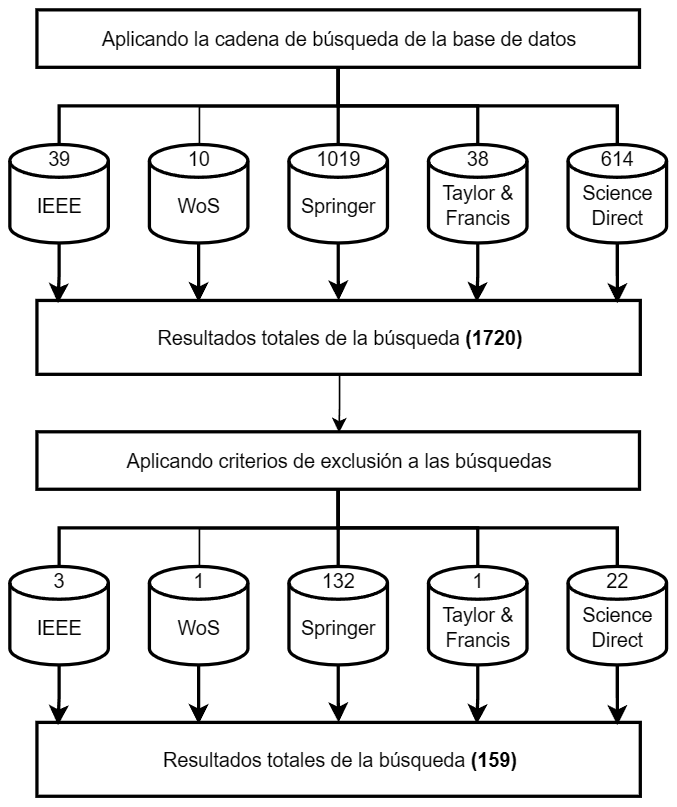
\includegraphics[width=0.7\textwidth]{mainmatter/II-desarrollo-metodologico/sms/imagenes/resumen-busqueda-bases.png}
	\caption{Diagrama resumen del proceso de búsqueda en bases de datos}
	\label{fig:resumen-busqueda-bases}
\end{figure}

\section{Eliminación de duplicados}\label{sec:eliminacion-duplicados}

La eliminación de estudios duplicados se llevó a cabo mediante la herramienta de gestión bibliográfica Mendeley. Tras la recopilación inicial, todos los registros fueron importados a dicha plataforma, la cual permitió la identificación y eliminación automática de publicaciones redundantes. Este proceso resultó en la exclusión de \textbf{tres} artículos duplicados, reduciendo el total de estudios a 156. La \autoref{fig:eliminacion-duplicados} presenta una representación gráfica de estos resultados.

\begin{figure}[H]
	\centering
	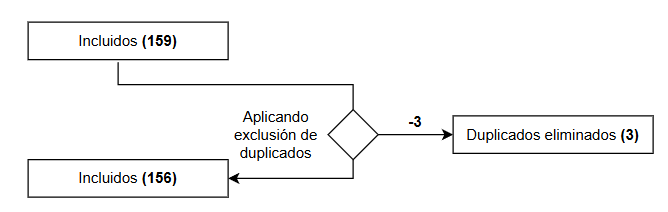
\includegraphics[width=0.9\textwidth]{mainmatter/II-desarrollo-metodologico/sms/imagenes/eliminacion-duplicados.png}
	\caption{Diagrama del proceso de eliminación de resultados duplicados}
	\label{fig:eliminacion-duplicados}
\end{figure}

\section{Priorización de estudios}\label{sec:priorizacion-estudios}

Tras la selección inicial de los artículos, se procedió al análisis de los campos \textit{title}, \textit{abstract} y \textit{keywords} de cada registro. Como resultado de esta revisión, se generaron métricas de calidad para cada artículo con el objetivo de priorizar aquellos más relevantes para la investigación. Las métricas empleadas fueron las siguientes:

\begin{itemize}
	\item \textbf{SCI} \textit{(Science Citation Index)}
	\item \textbf{CVI} \textit{(Core Value Index)}
	\item \textbf{IRRQ} \textit{(Index Relation Research Question)}
\end{itemize}

Este proceso inició con un total de 156 artículos, los cuales fueron evaluados en función de su alineamiento con los objetivos de la investigación. La fase de \textit{screening} permitió descartar 139 estudios, ya que algunos abordaban herramientas tecnológicas en contextos distintos al de interés y otros no se encontraban alineados con los objetivos de investigación establecidos.

\section{Estrategia de búsqueda usando bola de nieve}\label{sec:bola-de-nieve}

En esta etapa, la estrategia de snowballing se aplicó a la totalidad de los 18 estudios elegidos (17 mediante el proceso de selección y uno incluido directamente), en lugar de limitarse a un grupo reducido de artículos semilla. Esta decisión amplió la cobertura de la revisión y redujo el riesgo de omitir literatura relevante, fortaleciendo la exhaustividad del protocolo.

En este proceso se aplicaron las estrategias de bola de nieve directa \textit{(forward)} e inversa \textit{(backward)}, con el objetivo de identificar literatura adicional relevante que no hubiera sido recuperada durante la búsqueda automática en las bases de datos. La búsqueda por bola de nieve inversa permitió identificar un estudio adicional, mientras que la búsqueda por bola de nieve directa permitió identificar tres estudios adicionales, lo que resultó en un total de cuatro estudios incorporados.

El resumen de este proceso puede observarse en la \autoref{fig:proceso-snowball}.

\begin{figure}[H]
	\begin{center}
		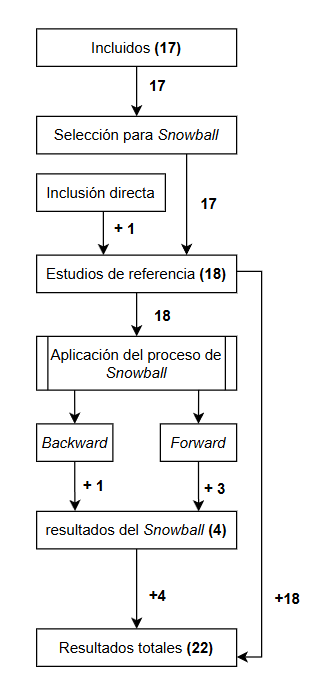
\includegraphics[width=0.4\textwidth]{mainmatter/II-desarrollo-metodologico/sms/imagenes/proceso-snowball.png}
	\end{center}
	\caption{Resumen del proceso de búsqueda por bola de nieve}
	\label{fig:proceso-snowball}
\end{figure}

\section{Identificación de estudios}
\subsection{Cuadro de estudios}

Los estudios resultantes del proceso de \ac{SMS} se presentan en la \autoref{tab:selected-primary-studies}.

\begin{table}[H]
	\centering
	\caption{Los 22 estudios primarios seleccionados (\acs{SPS}s)}
	\label{tab:selected-primary-studies}

	\fontsize{8pt}{10pt}\selectfont
	\renewcommand{\arraystretch}{1.2}

	\begin{tabular*}{\textwidth}{l @{\extracolsep{\fill}} r l @{\extracolsep{\fill}} r l @{\extracolsep{\fill}} r l @{\extracolsep{\fill}} r l @{\extracolsep{\fill}} r}
		\toprule
		\textbf{ID} & \textbf{Ref}   &
		\textbf{ID} & \textbf{Ref}   &
		\textbf{ID} & \textbf{Ref}   &
		\textbf{ID} & \textbf{Ref}   &
		\textbf{ID} & \textbf{Ref}
		\\
		\midrule
		SPS001      & \spsone        &
		SPS002      & \spstwo        &
		SPS003      & \spsthree      &
		SPS004      & \spsfour       &
		SPS005      & \spsfive
		\\
		SPS006      & \spssix        &
		SPS007      & \spsseven      &
		SPS008      & \spseight      &
		SPS009      & \spsnine       &
		SPS010      & \spsten
		\\
		SPS011      & \spseleven     &
		SPS012      & \spstwelve     &
		SPS013      & \spsthirteen   &
		SPS014      & \spsfourteen   &
		SPS015      & \spsfifteen
		\\
		SPS016      & \spssixteen    &
		SPS017      & \spsseventeen  &
		SPS018      & \spseighteen   &
		SPS019      & \spsnineteen   &
		SPS020      & \spstwenty
		\\
		SPS021      & \spstwentyone  &
		SPS022      & \spstwentytwo
		\\
		\bottomrule
	\end{tabular*}
	\vspace{5pt}
\end{table}


\subsection{Artículos por año y métricas}

A continuación se presentan las gráficas de los resultados de la búsqueda. En la \autoref{fig:sps-anios} se muestra la relación entre la cantidad de estudios por año y las métricas definidas en la \autoref{sec:priorizacion-estudios}.

\begin{figure}[H]
	\begin{center}
		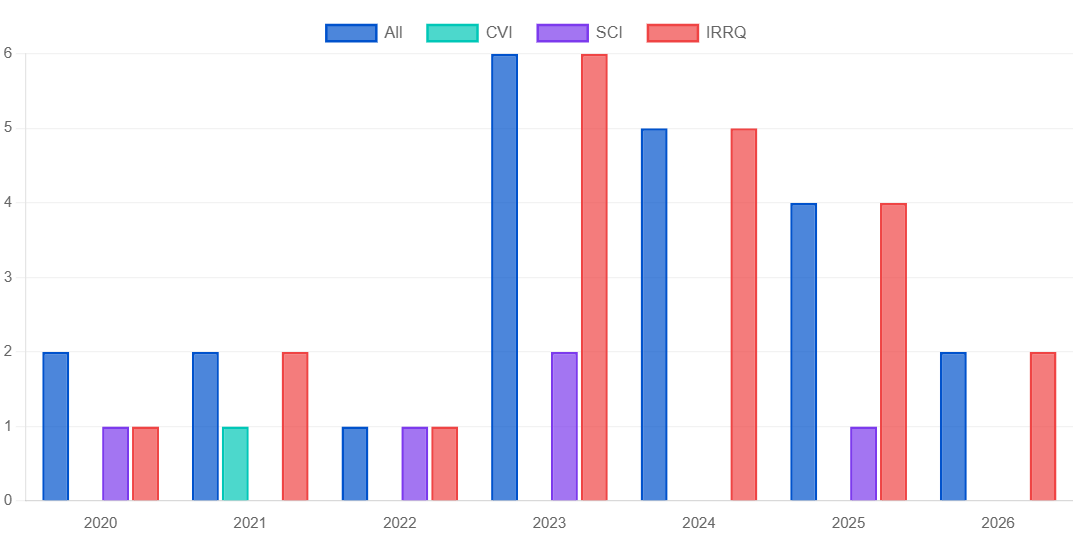
\includegraphics[width=0.8\textwidth]{mainmatter/II-desarrollo-metodologico/sms/imagenes/sps-anios.png}
	\end{center}
	\caption{Cantidad de artículos en conformidad con las métricas de calidad definidas en la \autoref{sec:priorizacion-estudios}}
	\label{fig:sps-anios}
\end{figure}

\subsection{Diferencias entre estrategias}

En la \autoref{fig:grafica-estrategia-vs-articulos} se puede observar el porcentaje de artículos obtenidos por cada estrategia.

\begin{figure}[H]
	\centering
	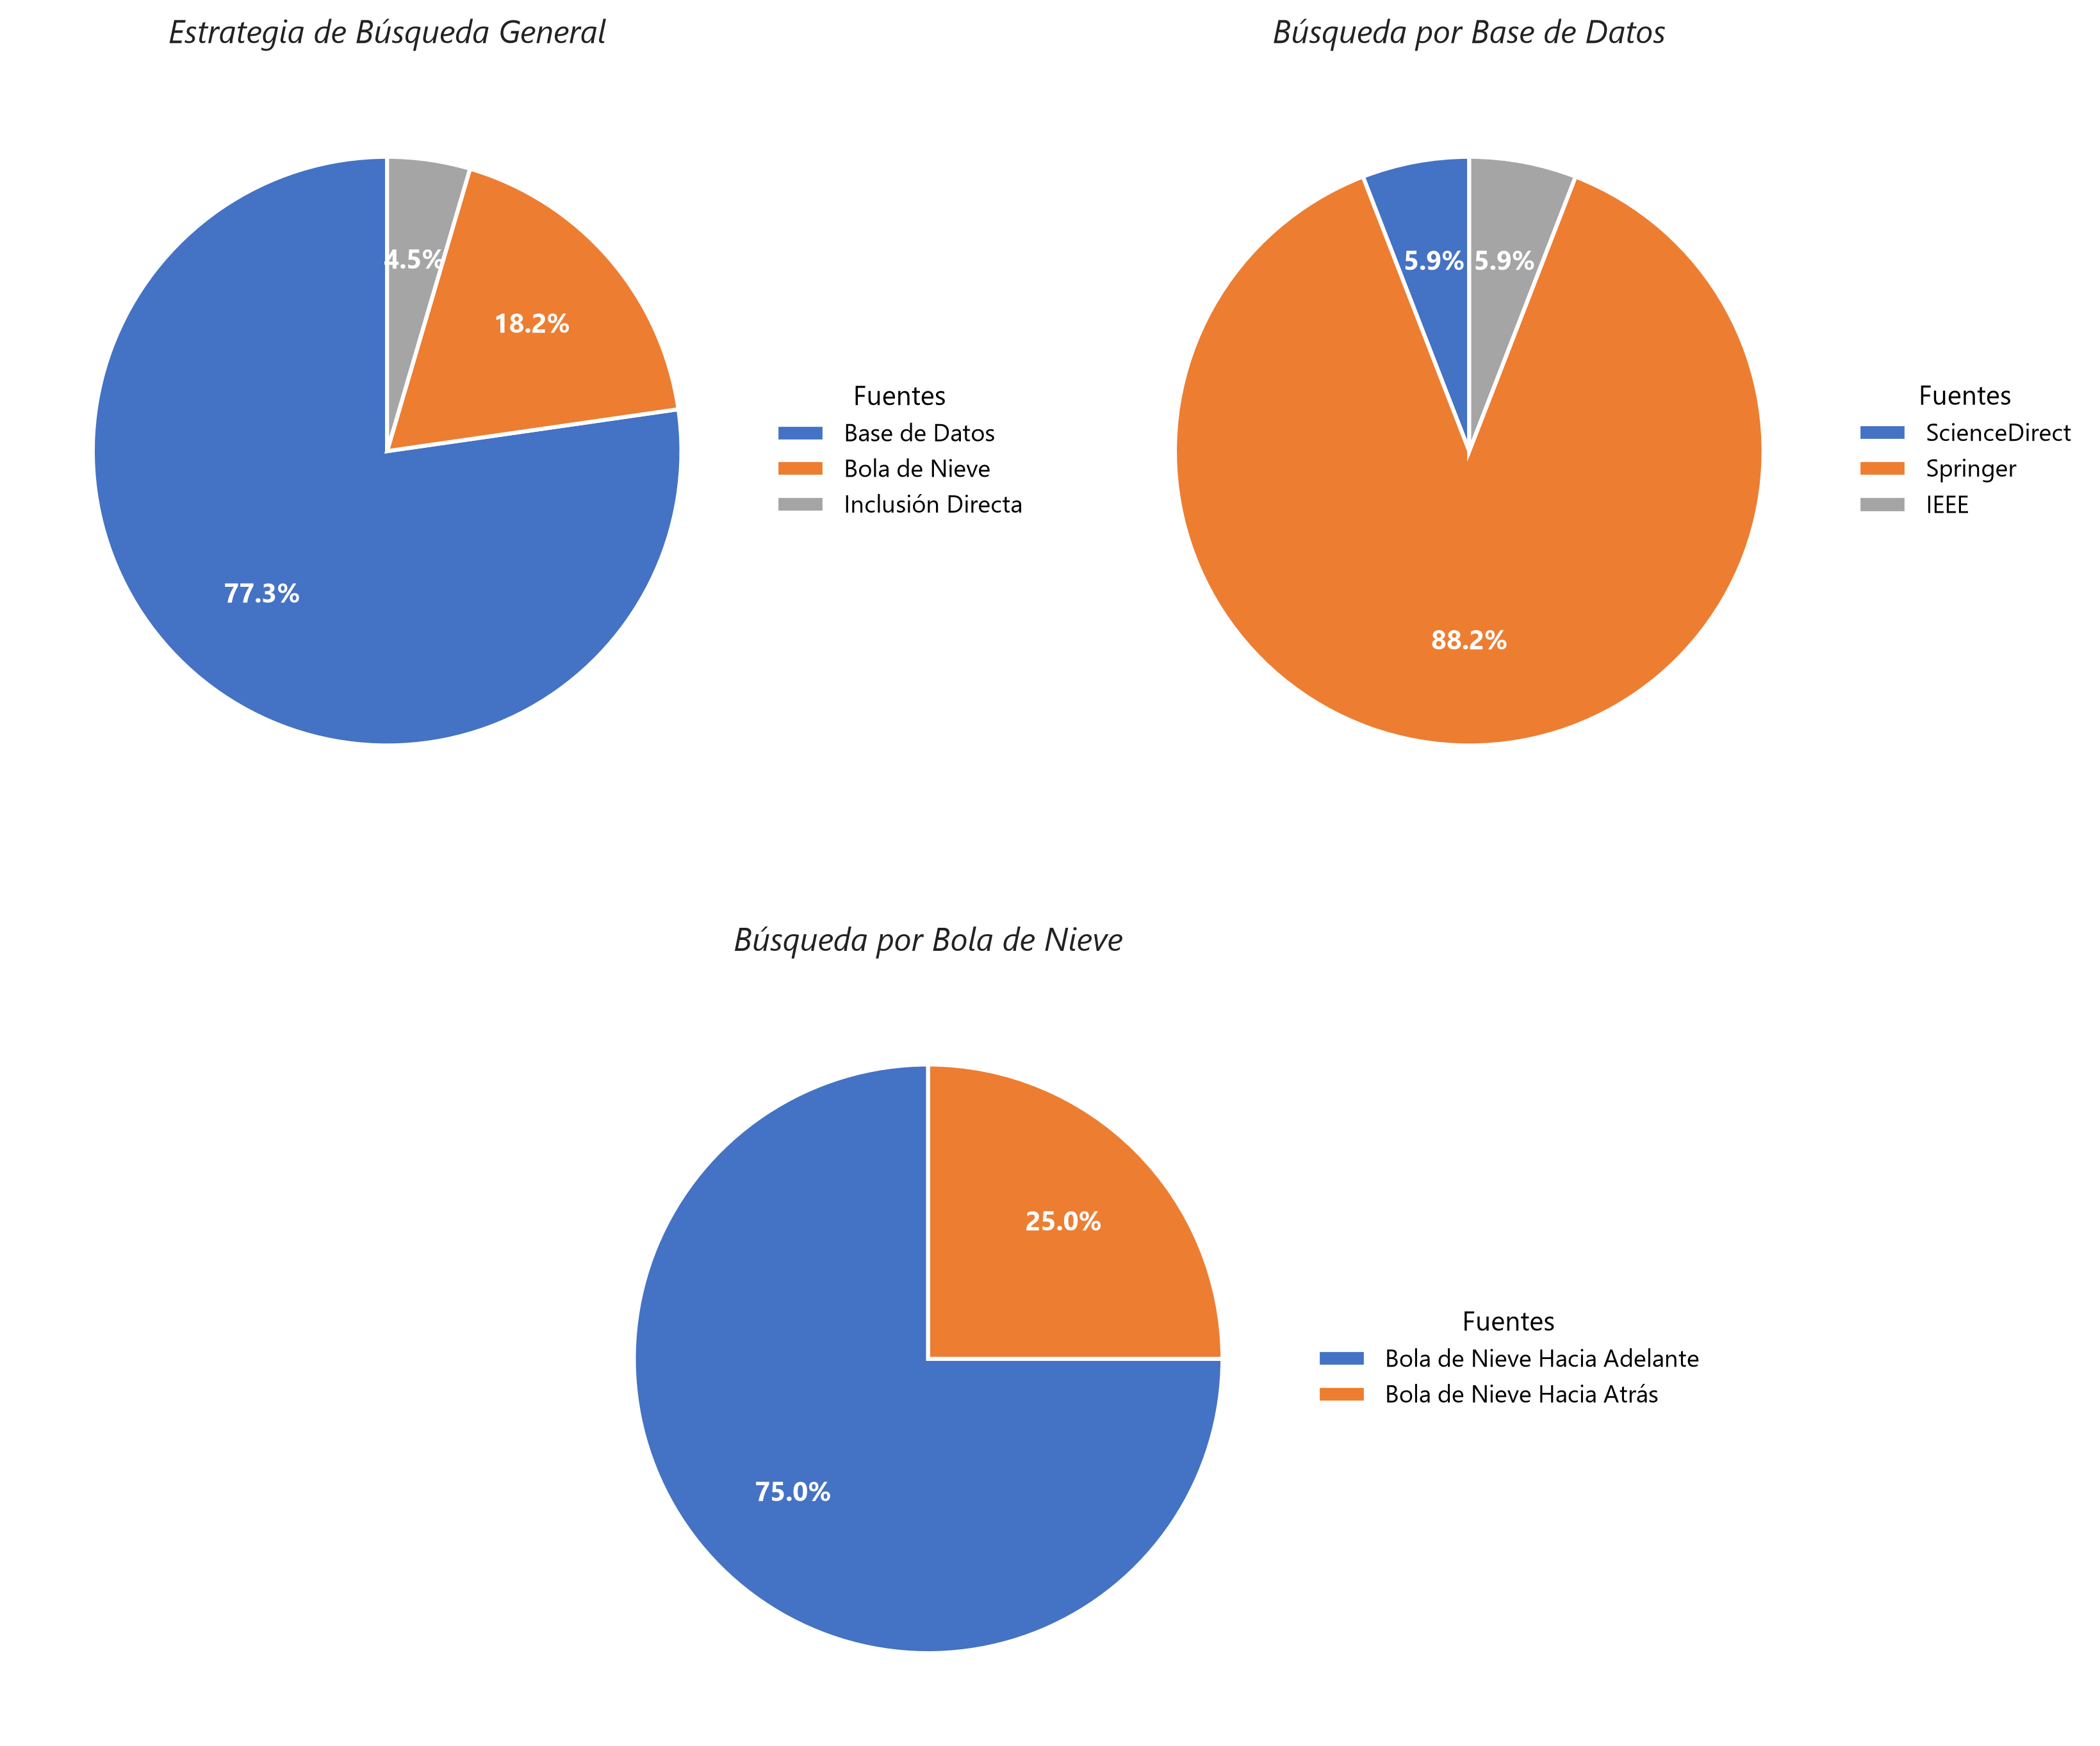
\includegraphics[width=0.8\textwidth]{mainmatter/II-desarrollo-metodologico/sms/imagenes/grafica-estrategia-vs-articulos.png}
	\caption{Porcentaje de artículos obtenidos por cada estrategia de búsqueda utilizada en el \acs{SMS}}
	\label{fig:grafica-estrategia-vs-articulos}
\end{figure}

\subsection{Tópicos frecuentes en los estudios}

Con el fin de caracterizar el enfoque temático de la literatura seleccionada, se analizaron los campos \textit{abstract} y \textit{keywords} de los 22 estudios incluidos en el mapeo. Este análisis permitió identificar y agrupar los principales temas de investigación presentes en los estudios, proporcionando una visión general de las áreas que han recibido mayor atención en la literatura. Los resultados de esta clasificación se muestran en la \autoref{fig:grafica-topicos}.

\begin{figure}[H]
	\centering
	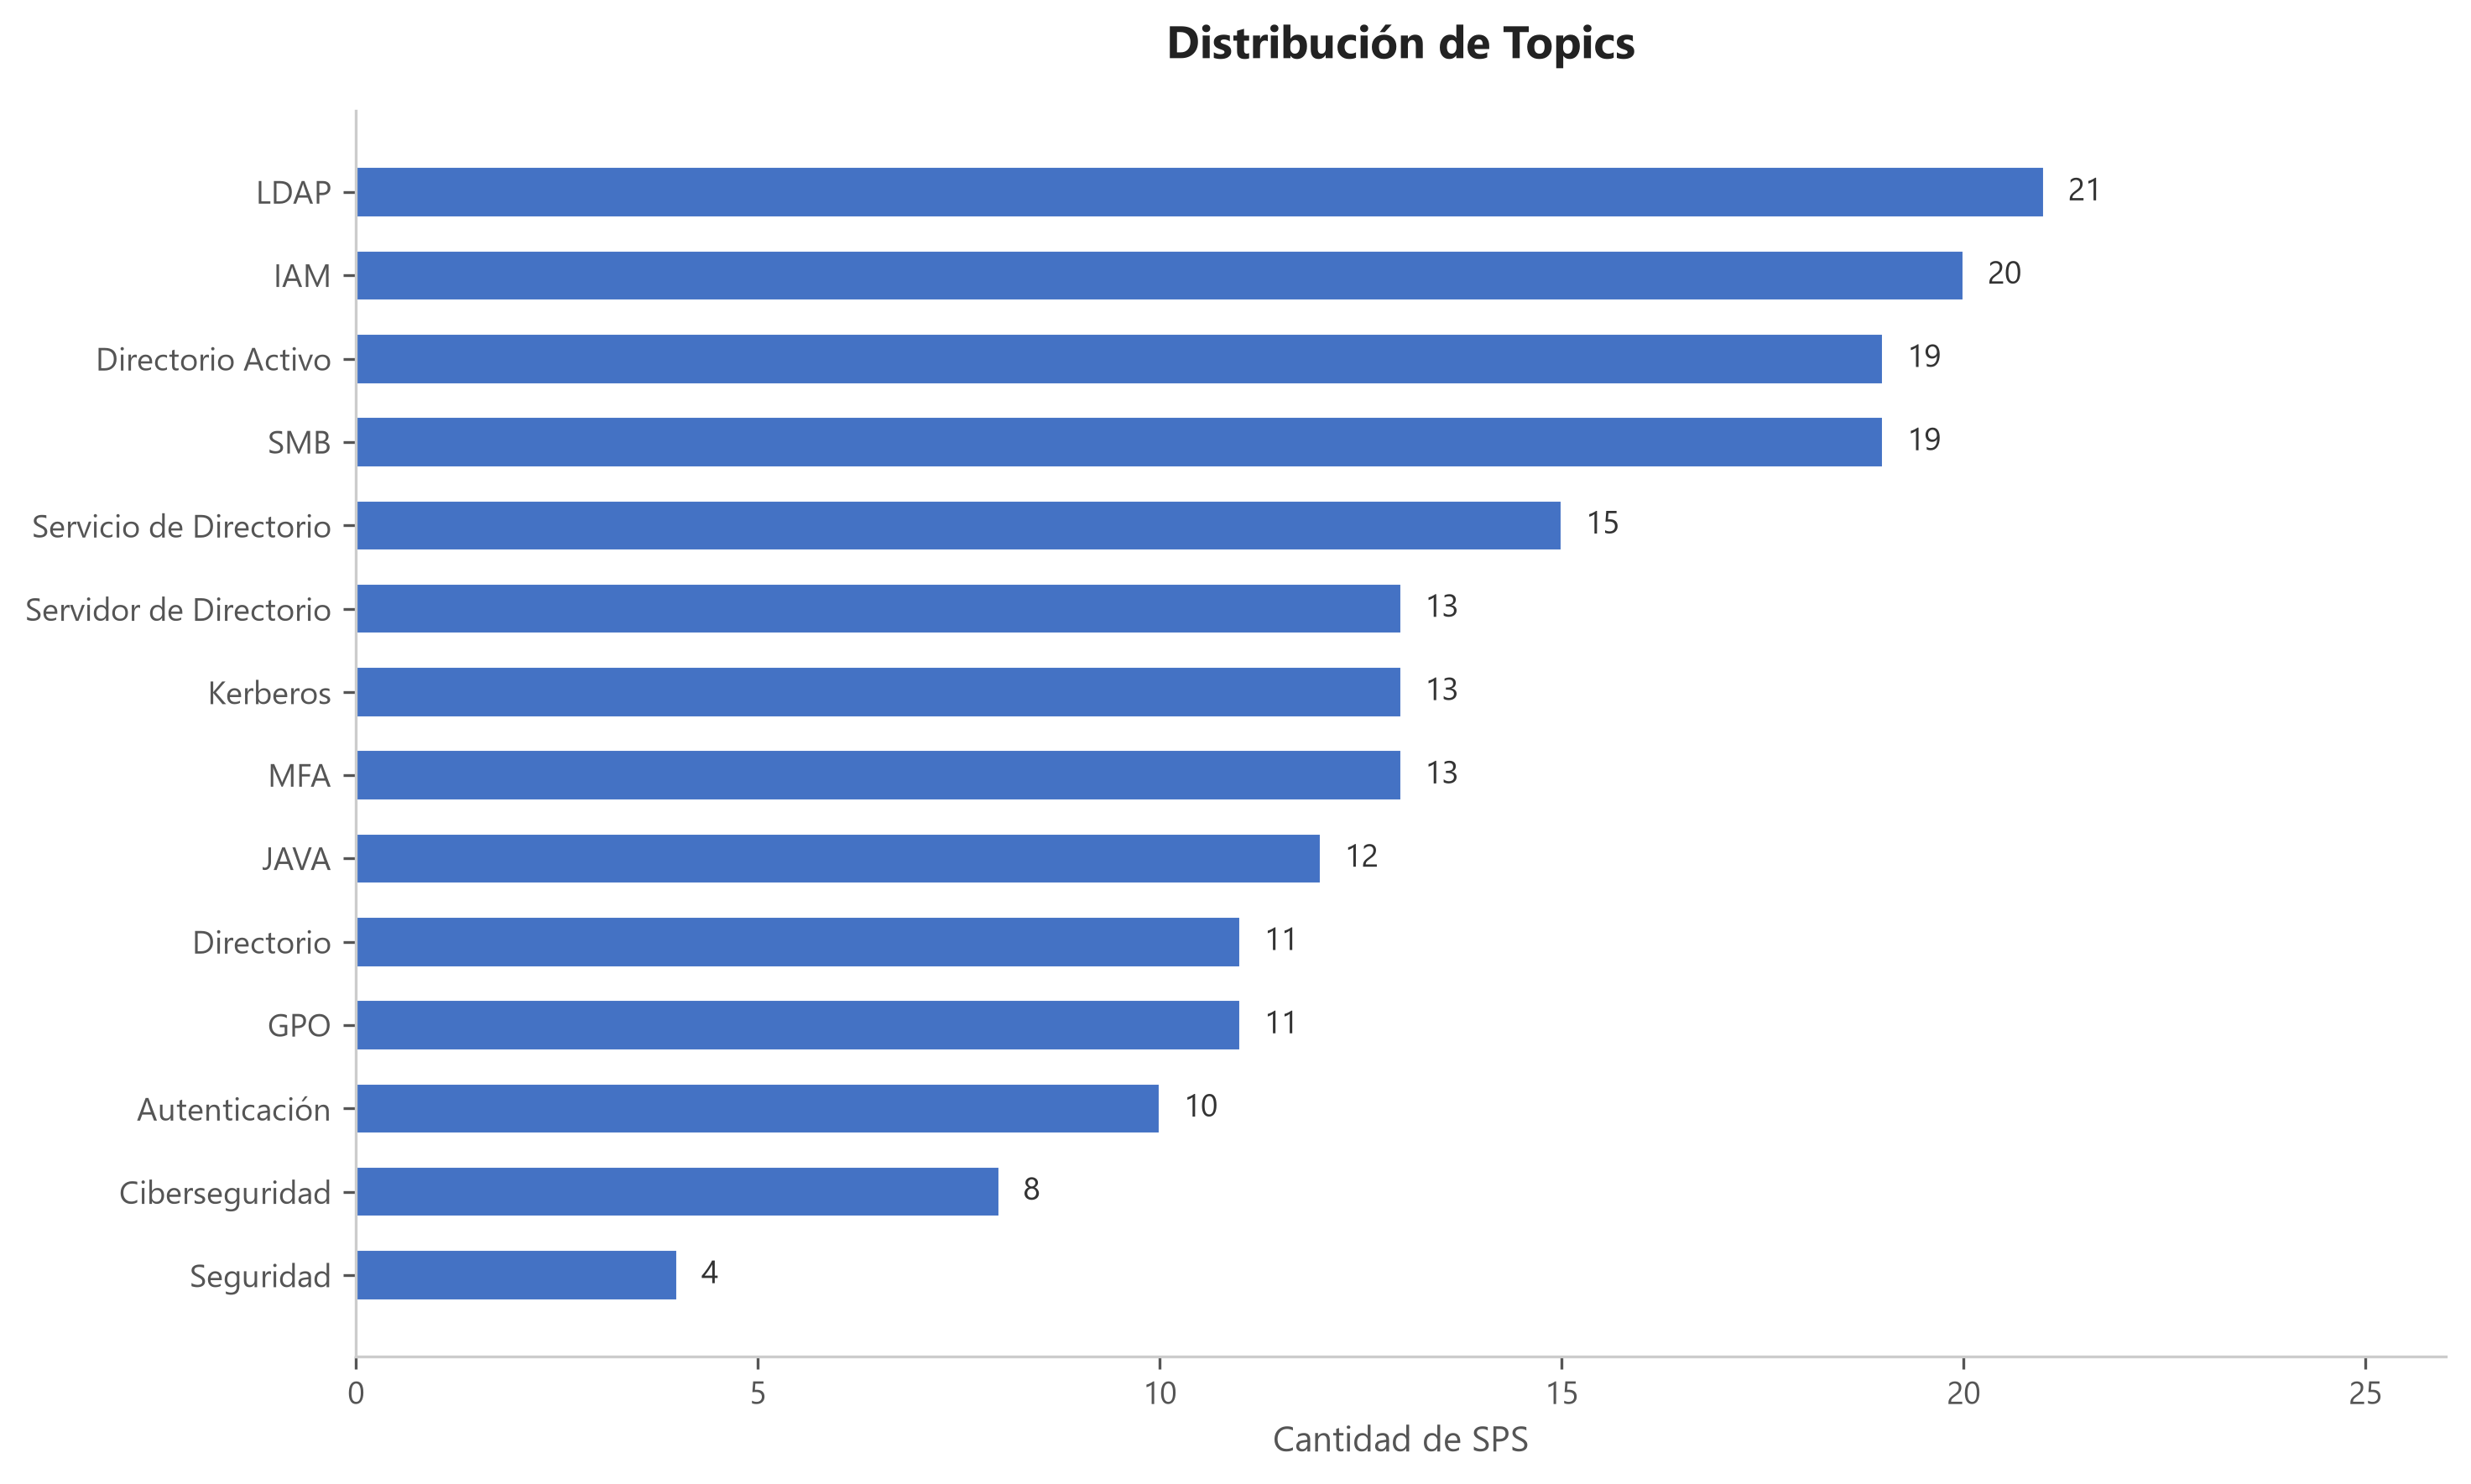
\includegraphics[width=0.9\textwidth]{mainmatter/II-desarrollo-metodologico/sms/imagenes/grafica-topicos.png}
	\caption{Diagrama de la distribución de los tópicos}
	\label{fig:grafica-topicos}
\end{figure}

\subsection{Conformidad con las preguntas de investigación}

Con respecto al cumplimiento de las preguntas de investigación definidas en la \autoref{subsubsec:rq-def}, se observó que la totalidad de los 22 estudios seleccionados aportó evidencia para responder la \textbf{RQ1}, lo que evidencia una cobertura completa de esta dimensión dentro del corpus analizado. Por su parte, 21 de los 22 estudios contribuyeron a responder la \textbf{RQ2}, indicando que esta temática también presenta una alta representación en la literatura considerada, aunque con un alcance ligeramente menor.

Estos resultados ponen de manifiesto una estrecha relación entre los objetivos de investigación planteados y los estudios finalmente incluidos en el mapeo sistemático, lo que respalda la pertinencia del proceso de selección aplicado. La distribución y el grado de solapamiento entre ambas preguntas de investigación se presentan en la \autoref{fig:grafica-venn-rqs}.

\begin{figure}[H]
	\centering
	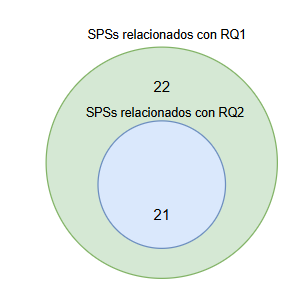
\includegraphics[width=0.4\textwidth]{mainmatter/II-desarrollo-metodologico/sms/imagenes/grafica-venn-rqs.png}
	\caption{Diagrama de los \acs{SPS}s relacionados con cada pregunta}
	\label{fig:grafica-venn-rqs}
\end{figure}

\section{Información de la herramienta}

La herramienta utilizada para este proceso de revisión de la literatura fue \textbf{SMS-BUILDER}, desarrollada por el Dr. Christian Andrés Candela Uribe la cual se encuentra disponible en \textit{Docker Hub}. La imagen puede consultarse en el siguiente enlace:

\begin{center}
	\href{https://hub.docker.com/r/griduq/sms-builder}{\texttt{https://hub.docker.com/r/griduq/sms-builder}}
\end{center}

\section{Reproducibilidad del método}

Con el fin de fomentar la reproducibilidad del método de revisión, se proporciona el mecanismo de verificación que permite a los revisores y lectores acceder de forma transparente a la información utilizada, generada mediante la herramienta \acs{SMS}-Builder de \citet{SMSBuilder2020}.

\begin{itemize}
	\item Imagen Docker disponible públicamente que integra toda la documentación necesaria para crear un contenedor con los datos del proceso:
	      \url{https://hub.docker.com/r/alejoosorio/sms-directory-service}.
\end{itemize}

\noindent
Adicionalmente, se implementaron procesos de respaldo como medida de seguridad. Estos \textit{backups} fueron almacenados en ubicaciones diferentes, siguiendo la estrategia de respaldo \textbf{3--2--1}.

\section{Conclusiones de la revisión sistemática de la literatura}

La presente revisión sistemática de la literatura abordó de manera rigurosa la identificación, selección y análisis de la evidencia científica relacionada con el dominio de estudio definido. Mediante la aplicación de una estrategia de búsqueda estructurada, complementada con técnicas de \textit{snowballing} y criterios de inclusión y exclusión previamente establecidos, fue posible conformar un conjunto final de 22 estudios relevantes para la investigación.

El análisis de los estudios seleccionados caracterizó el estado actual de la literatura, trazó las principales líneas de investigación abordadas por la comunidad científica y determinó el grado de cobertura de las preguntas de investigación planteadas. Los resultados obtenidos evidencian correspondencia entre las preguntas de investigación planteadas y la literatura recuperada, ya que la totalidad de los estudios contribuyó a responder la \textbf{RQ1}, mientras que la gran mayoría aportó evidencia para la \textbf{RQ2}.

Asimismo, el proceso de revisión consolidó una visión estructurada del área de investigación, identificando tendencias, enfoques y características comunes presentes en los trabajos analizados. Los hallazgos obtenidos sirven como referencia para el desarrollo de las etapas posteriores de la investigación, al aportar evidencia sobre el estado del arte del área estudiada.

\section{Tecnologías}\label{sec:tecnologias}

\subsection{Tecnologías identificadas}\label{subsec:tecnologias-identificadas}

Como resultado del proceso de búsqueda, selección y extracción de información se identificaron cuatro alternativas de software libre y de código abierto relacionadas con servicios de directorio.

Las tecnologías identificadas fueron:

\subsubsection{OpenLDAP}

OpenLDAP fue identificado como una de las alternativas de código abierto para la implementación de servicios de directorio. Según la documentación oficial del proyecto, se trata de una implementación de código abierto del protocolo \acs{LDAP}, orientada a entornos distribuidos y distribuida bajo la OpenLDAP Public License, una licencia libre de carácter permisivo con características similares a las licencias \ac{BSD} \citep{OpenLDAP2026}.

\subsubsection{389 Directory Server}

389 Directory Server fue identificado como una alternativa orientada a despliegues de mayor escala, incluyendo entornos corporativos y académicos. De acuerdo con la documentación oficial del proyecto, se trata de un servicio de directorio de nivel empresarial cuyo esquema de licenciamiento contempla una \acs{GPL} Exception y componentes distribuidos bajo Apache 2.0 y \acs{LGPL} para determinados elementos y extensiones \citep{DS3892026}.

\subsubsection{ApacheDS}

Apache Directory Server (ApacheDS) constituye una alternativa desarrollada en Java bajo el proyecto Directory de la Apache Software Foundation. Conforme a su documentación oficial, la solución se distribuye bajo Apache License 2.0 \citep{ApacheDS2026}.

\subsubsection{OpenDJ}

OpenDJ corresponde a una alternativa cuyos orígenes se remontan a los desarrollos de Sun Microsystems y ForgeRock, y que actualmente continúa su desarrollo por medio de la comunidad Open Identity Platform. La solución se distribuye bajo la \ac{CDDL} \citep{OpenDJ2026}.

\section{Incorporación de tecnología adicional}\label{sec:incorporacion-tecnologia-adicional}

Los resultados obtenidos mediante el \ac{SMS} permitieron establecer cuatro alternativas tecnológicas relacionadas con los servicios de directorio: OpenLDAP, 389 Directory Server, ApacheDS y OpenDJ. Estas alternativas constituyeron el resultado de la búsqueda y selección bibliográfica realizada mediante el protocolo definido para el SMS.

De manera complementaria, se incorporó FreeIPA al conjunto de alternativas consideradas para la evaluación tecnológica. Esta incorporación no corresponde a un resultado del SMS, sino a una decisión metodológica posterior orientada a ampliar el conjunto de alternativas disponibles para el análisis comparativo. Por tanto, FreeIPA se mantuvo diferenciada de las tecnologías identificadas mediante el proceso de revisión sistemática.

La incorporación de FreeIPA se fundamentó en su correspondencia con las necesidades y requisitos definidos para el servicio de directorio. De acuerdo con la documentación oficial del proyecto, FreeIPA integra componentes orientados a la gestión centralizada de identidades, autenticación, políticas y servicios de directorio \citep{FreeIPA2026}. Estas características presentan correspondencia con los requisitos establecidos para la solución propuesta y justifican su consideración como alternativa tecnológica adicional en la etapa de evaluación.

La incorporación de FreeIPA permite ampliar el conjunto de alternativas tecnológicas que serán sometidas posteriormente al proceso de evaluación, manteniendo diferenciada su procedencia respecto de las tecnologías identificadas directamente en el mapeo.

\section{Conjunto de tecnologías candidatas}\label{sec:conjunto-tecnologias-candidatas}

Como resultado de la identificación realizada mediante el \ac{SMS} y de la incorporación de la alternativa adicional, se estableció el siguiente conjunto de tecnologías candidatas, el cual se presenta en la \autoref{tab:tecnologias_candidatas}:

\begin{table}[htbp]
	\centering
	\caption{Conjunto de tecnologías candidatas.}
	\fontsize{9pt}{10pt}\selectfont
	\renewcommand{\arraystretch}{1.4} % Ajusta el espaciado vertical de las filas
	\begin{tabularx}{\textwidth}{|l|l|>{\raggedright\arraybackslash}X|}
		\hline
		\tableheader
		\multicolumn{1}{|c|}{\textbf{Tecnología}} &
		\multicolumn{1}{c|}{\textbf{Procedencia}} &
		\multicolumn{1}{c|}{\textbf{Licenciamiento}}
		\\
		\hline
		OpenLDAP                                  &
		Resultado del \acs{SMS}                   &
		OpenLDAP Public License
		\\
		\hline
		389 Directory Server                      &
		Resultado del \acs{SMS}                   &
		\ac{GPL} Exception / Apache 2.0 / \ac{LGPL}
		\\
		\hline
		ApacheDS                                  &
		Resultado del \acs{SMS}                   &
		Apache License 2.0
		\\
		\hline
		OpenDJ                                    &
		Resultado del \acs{SMS}                   &
		Common Development and Distribution License (\ac{CDDL})
		\\
		\hline
		FreeIPA                                   &
		Incorporación adicional                   &
		GNU General Public License v3 (GPLv3)
		\\
		\hline
	\end{tabularx}
	\label{tab:tecnologias_candidatas}
\end{table}


